\subsection*{Feedback loops and Ripples\label{sec:feedback-loop-and-ripples}}

%When there is a lack of input from customers/users, then someone has to decide.


A feedback loop exists when a decision maker experiences the harms and benefits of their decision. Decisions that lack a feedback loop still have consequences for the decision maker, in that potential future decisions are altered or limited\footnote{In~\cite{1983_Lipsky} Lipsky discusses feedback loops in chapter 4 page 40.}.


Virtuous cycles and vicious cycles are rare in bureaucratic organizations because there are rarely mechanisms for feedback loops. Instead, there are \glspl{ripple} -- propagation of consequences for other people's schedules, what is possible for other people, and dependent tasks to be carried out by people other than the decision maker.


The weak feedback mechanisms for a bureaucrat are reputation (subject to spin) and rarely enforced retroactive accountability -- what did you know and when did you know it.
%Reputation is social.
Retroactive accountability depends on written records from meeting notes, emails, agendas, and reports. Reducing the potential for retroactive accountability is one motive for bureaucrats avoiding written records for decisions and policies.


Because of the lack of quantitative feedback loops fir bureaucrats, there is significant interest in documenting justification, proactive monitoring, reporting, and retroactive assessment. Each of those activities creates more administrivia.


When there are multiple competing objectives among different stakeholders in a zero sum use of resources, how can you determine what's best? In some domains there are feedback loops to guide progress. When feedback loops are weak or not present, then the most powerful stakeholder (which is distinct from the biggest or loudest) will dominate. 


\ \\

% TODO: need a transition between topics

%****************************************
% https://graphthinking.blogspot.com/2020/01/hierarchy-of-justification.html

Ordering the quality of a justification
\begin{enumerate}
    \item I have no explanation.
    \item This is my opinion.
    \item We've always done it that way (a \href{https://en.wikipedia.org/wiki/Cargo_cult}{cargo cult}).
    \item Based on my experience.
    \item I was told to do it this way.
    \item I think this is the best way (no reasoning, but a desire to optimize; optimization criterion undefined).
    \item This way is most effective because X (not quantified, desire to optimize, has an optimization criterion).
    \item This way is most effective because X (quantified, desire to optimize, has an optimization criterion).
    \item This way is most effective because X compared to other options (quantified, desire to optimize, has an optimization criterion).
\end{enumerate}

%****************************************

\ \\

% TODO: need a transition between topics


\subsubsection*{Special interest groups}

Within bureaucratic organizations there are special interest groups that care about aspects of the shared resource central to the organization. 
When there is a benefit to a small group and the cost is to a larger group, inefficiency can occur.
% TODO? tie in with Public choice theory

The \href{https://en.wikipedia.org/wiki/Social_trap}{social trap} is ``a conflict of interest or perverse incentive where individuals or a group of people act to obtain short-term individual gains, which in the long run leads to a loss for the group as a whole."
The feedback loop for the diffused value is weaker than the feedback loop for the interest group. 

\subsubsection*{Spending taxpayer dollars}

As an example of a weak feedback loop, consider the scenario of a government employee deciding how to spend government money.

\marginpar{[Tag] Story Time; Math}
\index{story time!taxes and spending}
\begin{mdframed}
Suppose you earn \$100,000 and the tax rate is 30\%. Then your tax money sent to the government is \$30,000.
How does that compare to what the government collects in taxes?

For the United States, ``in 2021 the government collected \$4.05 trillion in revenue."
\footnote{source: Government Revenue | \href{https://datalab.usaspending.gov/americas-finance-guide/revenue/}{U.S. Treasury Data Lab}}

That means your taxes of \$30,000 would be
30000/4050000000000 = 0.00000074\% of the tax base for the country.

If you are a federal government bureaucrat and you do not maximize the effectiveness of spending \$1,000,000 of government money, of that misallocated money only \$0.0074, or about one penny, was taxes you paid. The financial feedback loop is weak.

Some federal government bureaucrat earn slightly more, so the cost of wasting \$1,000,000 is more significant.
Federal pay is limited to about \$220,000\footnote{Wikipedia entry on \href{https://en.wikipedia.org/wiki/Executive\_Schedule}{Executive Schedule}}, so that raises the feedback to 2 pennies.
\end{mdframed}

The lack of feedback allows waste to go unfelt. There's no immediate consequence for the decision maker.
%Waste is indistinguishable from not enough funding or insufficient skills.

\ \\

Example feedback loop:
\begin{center}
\begin{figure}[ht]
    \centering
    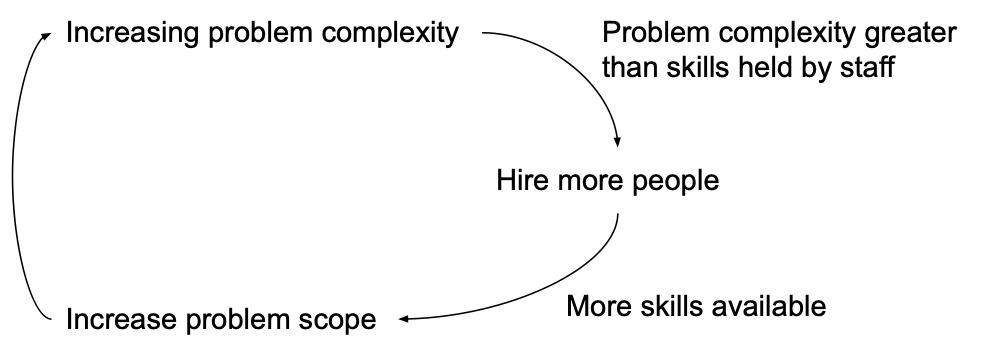
\includegraphics[width=0.8\textwidth]{images/feedback_loop_complexity_and_staffing}
    \caption{Complexity requires more staffing; having more staff means more skills are available; under-utilized staff skills make room for more scope; more scope adds to complexity.}
    \label{fig:complexity_and_staff_growth}
\end{figure}
\end{center}

\subsubsection{Example feedback loop: Security agent making a fair decision}
% https://graphthinking.blogspot.com/2017/09/a-simple-illustration-of-bureaucracy.html
\marginpar{[Tag] Story Time}
\index{story time!airport security}
\begin{mdframed}
I was going through passport control. 
There was a \href{https://en.wikipedia.org/wiki/Transportation_Security_Administration}{TSA officer} directing people into one of two lines. Both lines were long. The lines were not of equal length. Both lines terminate at a bunch of passport checking agents. Each passport check takes a minute. Passport checking TSA officers operate independently and concurrently.


The TSA officer's perspective is that there are two long lines. His procedure is two balance the two lines (for fairness). He does this by pointing people into one of the two lines, with his choice driven which line has room available.

Two people enter and are directed by the TSA officer. The first person is directed left, the second goes right. The TSA officer's job is completed.

The person in the left line finishes 5 minutes before the person in the line on the right. This difference in completion time is frustrating is frustrating for the person who is in the line on the right.

Because the lines are not of equal length, balancing the start of the line is an suboptimal method. The consequence is that what seems fair to the TSA officer ends up not being fair for people going through the line. The TSA officer had incomplete information -- the lines are not of equal length. Because the TSA officer isn't exposed to the consequence of is approach, he doesn't get feedback on whether it is suboptimal or not.
\end{mdframed}

Lesson: if the people making decisions do not experience the consequences of those decisions, then they have no incentive to improve decision making.

The person in the longer line feels frustrated. The negative feeling is due to a sense of powerlessness, and that the situation is recurring, and a better solution is available.

The optimal solution in this situation is to have a single line feeding the multiple TSA passport checkers. This eliminates the need for the decision maker.


\subsubsection{Parking garage}
% source: 
% https://graphthinking.blogspot.com/2019/07/altering-feedback-loops-to-change.html

\marginpar{[Tag] Story Time}
\index{story time!parking garage}
\begin{mdframed}
Bob parks his car in a parking garage every day. 
The parking garage owner charges \$20 per day for people to park their car.

Bob recently found that one of the exit gates for the parking garage is broken. If Bob uses that gate to leave the parking garage, the gate does not function and Bob cannot exit. Then Bob has to call the parking gate operator to request an exception (which is granted) and Bob can then exit that gate, avoiding the \$20/day charge.

This action (go to broken gate, request exception, avoid charge) has been repeated for a long time (months). Bob's motive is to avoid the \$20 parking charge; the cost is a mere phone call and a minor delay. This cheating behavior harms the parking garage owner's income. However, the parking gate operator, serving as intermediary, insulates the parking garage owner from the interaction with the cheater. The cheating behavior is small enough that the parking garage owner may not notice.
\end{mdframed}
